
\section{Mile's heuristics}
\subsection{Navigation}
\label{Navigation}
\begin{table}[H]
  \begin{center}
    \label{tab:table1}
    \begin{tabular}{||l|c|p{8cm}||} % <-- Alignments: 1st column left, 2nd middle and 3rd right, with vertical lines in between
      \textbf{Heuristic} & \textbf{Score} & \textbf{Comment}\\
      
      \hline
      Interaction Consistency & 4.5 & The website has a good interaction structure reflected in the pages of the same type. Elements as header, topbar and footer are present in every screen. There could be more consistency in links shape.\\
      \hline
      Group Navigation & 4.5 & Navigation from a list of items to its members is acceptably easy and intuitive, as well as between group members and from group member to the list.\\
      \hline
      Structural Navigation & 4 & It's acceptably intuitive between the components of a topic, well enough described and presented; it would have been more appropriate if it were equable between the sections.\\
      \hline
      Semantic Navigation & 3.5 & Even if there are almost always links to related contents, navigation between related topics is not always accessible in both directions.\\
      \hline
      Landmarks & 3.5 & Present in the various pages of the website but which do not always identify clear and easy-to-read references.\\

    \end{tabular}
  \end{center}
\end{table}
\medskip

\textbf{Interaction Consistency}\par
The website offers a significant experience due to interaction structure reflected in the pages of the same type. As a matter of fact, its structure is based on some elements available in each page: 
\begin{itemize}
\item \textbf{Header} (figure \ref{Header}): it links to different pages. In particular it allow users to navigate on:
\begin{itemize}
\item Company's \textbf{social network profiles} (\textit{Facebook, Twitter, Instagram and Linkedin});
\item \textbf{News section} for incoming report regarding Moviri;
\item \textbf{Contact section} due to interact with Moviri's employees;
\item \textbf{Moviri Careers}. It's a secondary website of Moviri where there are information regarding job opportunities;
\end{itemize}
\item \textbf{Topbar} (figure \ref{topbar}): allows a user to surf in each section of the website. In addition provides a search function for any content; 
\item \textbf{Footer} (figure \ref{Footer}): provides the same links to different sections of topbar and header, but at the foot of each page;
\end{itemize}
At the end, there could be more consistency in links shape.	


\begin{figure}[H]
  \centering
  \makebox[\linewidth]{
    
\includegraphics[scale=0.35]{images/header.png}}
  \caption{Header.}
   \label{Header}
\end{figure}

\begin{figure}[H]
  \centering
  \makebox[\linewidth]{
    
\includegraphics[scale=0.35]{images/topbar.png}}
  \caption{Topbar.}
   \label{topbar}
\end{figure}

\begin{figure}[H]
  \centering
  \makebox[\linewidth]{
    
\includegraphics[scale=0.35]{images/footer.png}}
  \caption{Footer.}
   \label{Footer}
\end{figure}
\medskip

\textbf{Group Navigation}\par
The navigation between the various components of a topic is intuitive, thanks to the good arrangement of the parts, that almost always have a title, an image and a short description. However, structural navigation slightly changes between the various sections. For instance, in the \textit{Business Lines} section each topic is represented by the combination of image and description side by side and unpaired with respect to the next one, while in the \textit{Resource} section each item is placed in a grid (fig. \ref{grid}) with its title and a respective image.
\medskip


\begin{figure}[H]
\centering
\begin{minipage}{.5\textwidth}
  \centering
  
\includegraphics[scale=0.30]{images/structural_navigation.png}
    \caption{Items in the Resource section.}
  \label{grid}
\end{minipage}%
\begin{minipage}{.5\textwidth}
  \centering
  
\includegraphics[scale=0.35]{images/structural_navigation_2.png}
        \caption{Items in the Business Lines section.}
\end{minipage}
\end{figure}


\textbf{Structural Navigation}\par
Thanks to components such as topbar and footer, it's possible to navigate between each section through links. The fact that links are placed both high and low helps user’s experience to be more intuitive, since it is not possible to go to the previous or next page. Anyway, the Structural Navigation along each page is always easily feasible and understandable.
\medskip






\textbf{Semantic Navigation}\par
Navigation between pages of different sections is easily allowed by topbar and footer. Nevertheless, there are situations in which this is not reversible. In particular this is not possible in the \textit{Resource} section after the click of an item; in fact, it redirects to pages of other websites leaving Moviri domain. It's sufficient to go back with the undo function of the browser, but could be quite uncomfortable.
\medskip

\textbf{Landmarks}\par
Landmarks cover all major contents of the website and they can be found both top and bottom part of the website in each section; Anyway, they could be improved to be more clear, evident and easily readable (fig. \ref{landmarks}). It’s always possible to be redirect to the homepage but the reference is not immediately understandable for a user visiting the website for the first time, considering that it is not identified with the well recognized term \textbf{“Home”}.

\begin{figure}[H]
  \centering
  \makebox[\linewidth]{
    
\includegraphics[scale=0.35]{images/Landmarks.png}}
        \caption{Landmarks.}
\label{landmarks}
\end{figure}

\subsection{Content}
\begin{table}[H]
  \begin{center}
    \label{tab:table1}
    \begin{tabular}{||l|c|p{8cm}||} % <-- Alignments: 1st column left, 2nd middle and 3rd right, with vertical lines in between
      \textbf{Heuristic} & \textbf{Score} & \textbf{Comment}\\
      
      \hline
     Information Overload & 4.5 & Information clearly distributed and organized in a minimalist way almost in all pages.\\
     
    \end{tabular}
  \end{center}
\end{table}
\medskip
\textbf{Information Overload}\par
Each information, both graphical and textual, is well balanced in each section of the website. This is one of the strength of website, even if in some sections the minimalism appears too grave and risks leading to a lack of information.

\subsection{Layout}
\label{Layout}

\begin{table}[H]
  \begin{center}
    \label{tab:table1}
    \begin{tabular}{||l|c|p{8cm}||} % <-- Alignments: 1st column left, 2nd middle and 3rd right, with vertical lines in between
      \textbf{Heuristic} & \textbf{Score} & \textbf{Comment}\\
      
      \hline
      Text Layout & 4 & The text is readable and the font is appropriate in the various sections. Colour choice could be more improved.\\
      \hline
      Interaction Placeholder-Semiotics & 4 & Textual and visual labels are expressive and reflect a good interaction/effect aspect, excluded some cases in which there is an inappropriate response to that expected.\\
      \hline
      Interaction Placeholder-Consistency & 4 & Labels for interactive elements are well organized in term of position but the icon are not always consistent and can be slightly improved.\\
      \hline
      Spatial Allocation & 4 & Generally fine and appropriate allocation of contents in the various pages, amendable the organization of semantically-distant elements in some pages.\\
      \hline
      Consistency of Page Structure & 3 & Page structure of each topic is consistent among pages but refering to different groups we detected severe changes of structure.\\

    \end{tabular}
  \end{center}
\end{table}
\pagebreak

\textbf{Text Layout}\par
Textual contents are easy-to-read. This is thanks to the font used in each point which is always proportional to the importance of the information. For instance, title or quotes has a larger font then simple descriptions. About the choice for the colour of the font we note that, even if almost always it matches with the rest of the layout, in certain parts the choice of the colour in contrast with the background is not absolutely appropriate (fig. \ref{text}).
\medskip

\begin{figure}[H]
  \centering
  \makebox[\linewidth]{
    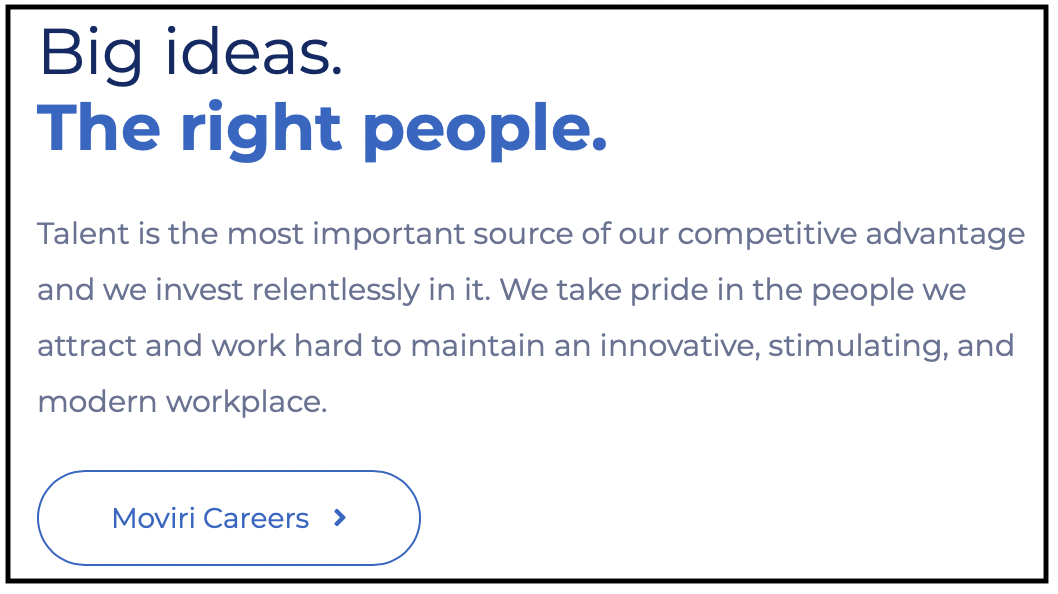
\includegraphics[scale=0.35]{images/text.png}}
  \caption{Part of the text layout in About page (from Moviri section).}
   \label{text}
\end{figure}


\textbf{Interaction Placeholder-Semiotics}\par
Textual and visual labels are expressive almost in every case. Only in few situations links are not visible by underling or a hand-cursor. In addition we found relevant issues characterized by a strange behaviour in some case, for instance clicking on partners image in the \textit{Business Line} section, as a result of which the page come back to the top of the page; moreover, this happens cliking on image. After all, labels of interactive elements are consistent and reflect acceptably good the interaction and the effect.\\

\medskip

\textbf{Interaction Placeholder-Consistency}\par
Considering the website in its integrity, it doesn’t show so many problems in terms of wording, icon and position, so, given its easy of use, we have not find relevant violations. 
Anyway we highlight 2 issues:
\begin{itemize}
\item The \textbf{Business Lines} doesn’t always work as homepage;
\item Even if the labels are well organized in term of position, the choice of the icon are not always consistent.
\end{itemize}
\medskip

\textbf{Spatial Allocation}\par
Each type of content is allocated spatially in an appropriate way respect to the relevance. Semantically related elements are close to each other but we would appreciate a better organization in the screen and spacing of semantically distant elements; in particular we refer, for example, to the “Industries” section: different items should be space out a little (fig. \ref{space}). 

\begin{figure}[H]
  \centering
  \makebox[\linewidth]{
    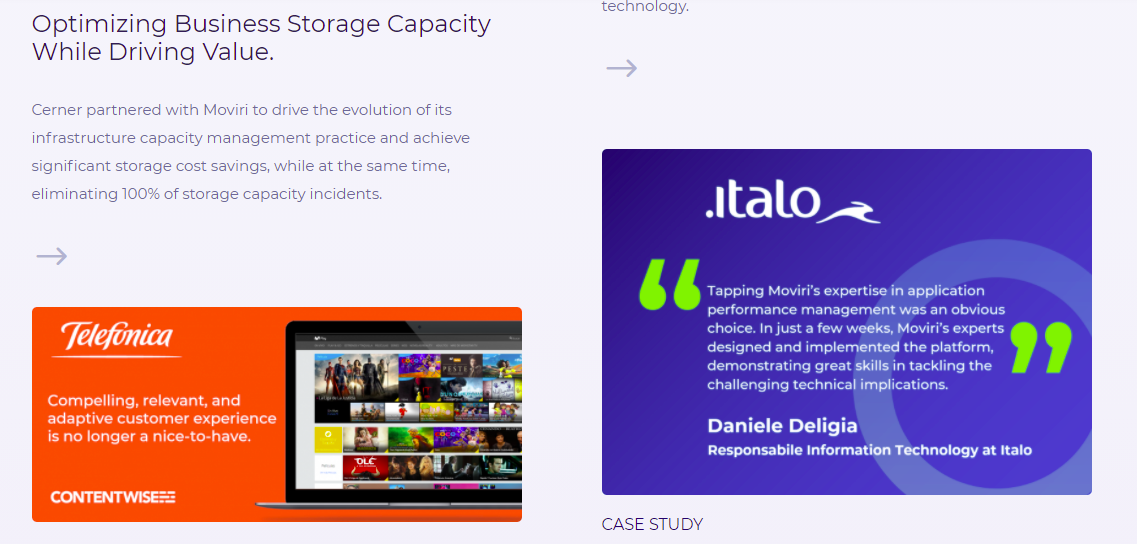
\includegraphics[scale=0.50]{images/spatial_allocation.png}}
    \caption{Industries section. In this section items are placed irregularly.}
    \label{space}
\end{figure}


\medskip
\textbf{Consistency of Page Structure}\par
Page structure of the topics is consistent among the pages, with few differences about contents allocation, but referring to different groups the structure often changes in a substantial way; anyway, in the resource section users can be redirected to other websites which have a completely different structure and font too, so they are absolutely not consistent, contrary to the topics of same sections.
\bigskip
\bigskip
\bigskip

\subsection{Nielsen's Heuristics}
\begin{table}[H]
  \begin{center}
    \label{tab:table1}
    \begin{tabular}{||l|c|p{8cm}||} % <-- Alignments: 1st column left, 2nd middle and 3rd right, with vertical lines in between
      \textbf{Heuristic} & \textbf{Score} & \textbf{Comment}\\
      
      \hline
      Visibility of system status & 2 & User is not correctly informed about the ongoing process and is not oriented in the web site tree.\\
      \hline
      Match between system and real world & 4 & The language used by the system is quite user friendly, not suitable for inexperienced users.\\
      \hline
      Consistency and Standards & 3.5 & Words and symbols used in the system are coherent in terms of consistency but not enough in terms of standards of use.\\
      \hline
      Error prevention & 4 & The minimalist and clear design prevent any kind of error but we would appreciate the use of link labels for a matter of semantic clarity.\\
      \hline
      Flexibility and efficiency of use & 5 & The system fully respects the Efficiency and Flexibility criteria, offering the user a high visit experience.\\
      \hline
      Aesthetic and minimalist design & 4.5 & The web site has an essential visual design with a basic but clear presentation of the content, amendable in some section.\\
    \end{tabular}
  \end{center}
\end{table}

\medskip

\textbf{Visibility of system status }\par
The system hardly ever informs the user about what is going on; in general there are not status bars or orientation info, that is only present is the labels of the current position of the user but not the ongoing process. The problem is expanded by the fact that some items, for example in the “Industries” section, are opened in another web page, without being able to understand what the starting page is and failing to go back.  
\medskip

\textbf{Match between system and real world}\par
What we detected is that the system uses a language acceptably understandable for the user profile that can visit the web site, with an exposure of the information that follows a logical and natural order. Whereas the web site is intended for a user with technical skills, terms and definition used are high specialized and hardly suitable for an unskilled user. 
\medskip

\textbf{Consistency and Standards}\par
The choose of words and symbols in the system is coherent in terms of consistency, following good a platform internal convention but some elements and definitions often don't follow basic standards of use; for example, what we didn’t appreciate is the lack of the internationally recognized key word \textbf{“Home”} replaced by \textbf{Business Lines}, that it doesn’t immediately identify well its use. 
\medskip

\textbf{Error prevention}\par
The system uses a minimalist and very clear design that prevents the user to avoid both slips and mistakes in the choice of the page to visit but, even if all the groups and section are nominated in a unique and precise way, it was useful the use of link labels that can introduce to the user the link meaning, avoiding any kind of error in advance. 
\medskip

\textbf{Flexibility and efficiency of use}\par
Efficiency of use is guaranteed by the presence in all the pages of the web site of interaction elements, clear landmarks placed in a comfortable and intuitive way; we didn’t denote a particular flexibility but this is not a disabling limit given to the fact that the user is well profiled and the system is quite good designed to satisfy him. 
\medskip

\textbf{Aesthetic and minimalist design}\par
The system, on almost all pages, keeps the content and visual design focused on the essential, with some exceptions: for example, the difference between the \textbf{"Industries”} (fig. \ref{ind}) and the \textbf{"Resources”} (fig. \ref{res}) groups is tangible, considering that in the latter there is a better distribution and proportion between the information presented; anyway, the visual elements on the interface support the user’s primary goals without ever falling into a flat design. 

\begin{figure}[H]
  \centering
  \makebox[\linewidth]{
    
\includegraphics[scale=0.50]{images/H8_Nielsen.png}}
    \caption{Industries section.}
    \label{ind}
\end{figure}


\begin{figure}[H]
  \centering
  \makebox[\linewidth]{
    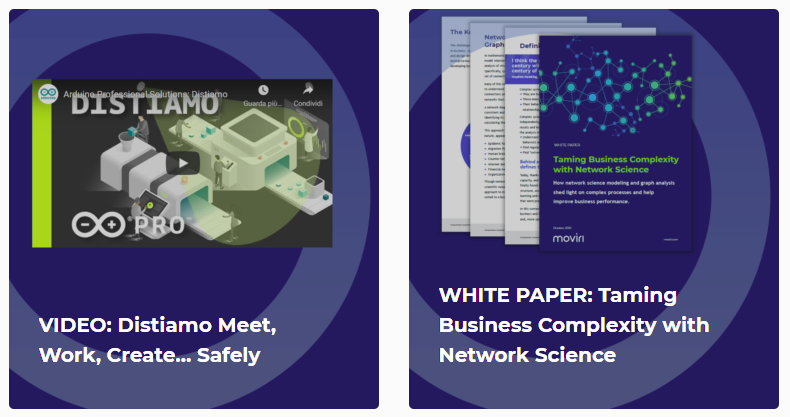
\includegraphics[scale=0.45]{images/H8_Nielsen_2.png}}
        \caption{Resources section.}
    \label{res}
\end{figure}
